\documentclass{beamer}
\usetheme{Madrid}
\usepackage{amsmath}
\usepackage{graphics}
\renewcommand{\bibname}{References}
\author{\bf{D. R. Upadhyay}}
\institute{Amrit Campus,TU}
\logo{
\includegraphics[height= 0.75cm]{logo.png}}
\title[SSTUL]{\Huge\bf{SSTUL
	}}
	\subtitle{A Presentation}
	\date{\today}
	\begin{document}
		\begin{frame}
			\begin{center}
				{\Huge\bf{ \color{blue}Webinar on\\\color{red}\LARGE``Scientific Writing Using LaTeX
					''}\\[0.2cm]
				\color{blue}\large  April 26, 2020 at \color{red}11:00 am (Nepali Time)\\[0.2cm]}
				
\includegraphics[height=2cm]{Tex}\\[0.1cm]
			\bf	\Large{\color{red}{Host: \color{blue}Devendra Raj Upadhyay}}
				\\Lecturer\color{blue}\\ Department of Physics\\ Amrit Campus, Tribhuvan University\\
			 Kathamndu, Nepal\\
			\end{center}
		\end{frame}
		
			\begin{frame}		
				\frametitle{\bf Outlines}
				\begin{itemize}
					\bfseries
			\item \color{red}Introduction
			\item \color{blue}Documents
			\item \color{red}Win edit
			\item \color{blue}Texmaker
			\item \color{red}TeXstudio
			\item \color{blue}JabRef
			\item \color{red}Applications
			\item \color{blue}Queries ???
						
				\end{itemize}	
			\end{frame}
			\begin{frame}		
		\frametitle{\bf Introduction(Cont..)}
		\begin{itemize}
			\bfseries
			\item \color{red}LaTeX is a high quality typesetting system which can produce
			modern technical and scientific documents such as Article, Report, Thesis,Term Paper, Project work, Book, and \color{violet}Beamer Presentation.\\
			\item \color{blue} Developed by Leslie B. Lamport (born February 7, 1941) is an American computer scientist.	\footnote{https://en.wikipedia.org/wiki/LaTeX(April, 2020)}\\
			\centering
	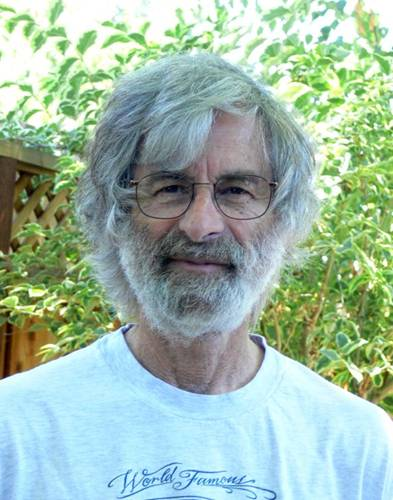
\includegraphics[height=4.5cm]{LM}\hspace{1cm}
	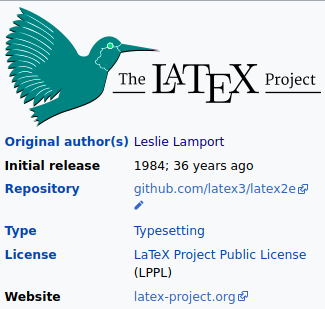
\includegraphics[height=4.5cm]{LA}
		
		\end{itemize}	
	\end{frame}


	\begin{frame}		
\frametitle{\bf Introduction(Cont..)}
\begin{itemize}
	\bfseries
	\item \color{red} Uses commands to create mathematical symbols.
	\item \color{blue}	Microsoft Word is based on a principle called \color{red}``What you see is what you get''(WYSIWYG),\color{blue} which means that the user immediately sees the document on the screen as it will appear on the printed page.
	 	\item \color{red} LaTeX is based on the principle of ``What you get is what you mean''(WYGIWYM), \color{blue} which implies that the document is not directly displayed on the screen and changes, such as format settings, are not immediately visible.\footnote{Knauff, M., \& Nejasmic, J., An Efficiency Comparison of Document Preparation Systems Used in Academic Research and Development. PloS one, 9(12), (2014).}
	\item \color{blue}The final document is obtained by converting the source file (.tex file) into a pdf file.
	\item \color{red} It is widely used in academia for the communication and publication
	of scientific and technical documents.
\end{itemize}
\end{frame}


	\begin{frame}		
		\frametitle{\bf Why not MS Word?}
	\bfseries \color{blue}
		\centering
		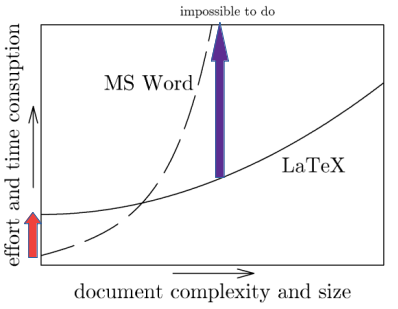
\includegraphics[width=8cm]{LW}
	\footnote{https://www.johndcook.com/blog/2008/04/03/microsoft-word-and-latex/}	
	\end{frame}


\begin{frame}
\frametitle{\bf Documents}
\begin{itemize}
	\bf 
\item \color{red}Article
\item \color{blue}Book
\item \color{red}Report
\item \color{blue}Thesis(Master, PhD)
\item \color{red}Term Paper
\item \color{blue}Manual
\item \color{red}Tech Report
\item \color{blue}Project Work
\item \color{red}Miscellaneous
\end{itemize}
\end{frame}

	\begin{frame}		
\frametitle{\bf Latex Documents}
\centering
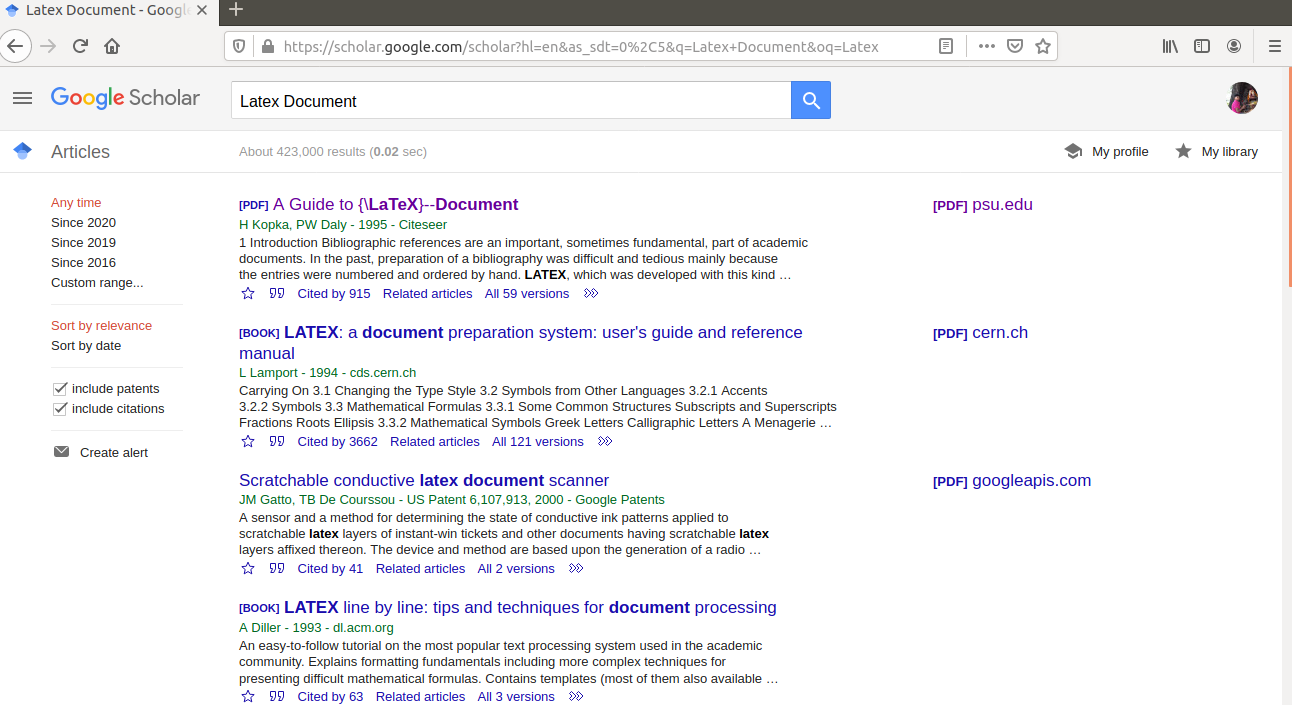
\includegraphics[width=12cm]{LD}
\footnote{https://scholar.google.com/(April, 2020).}	
\end{frame}

	\begin{frame}		
\frametitle{\bf Thesis(Cont..)}
\centering
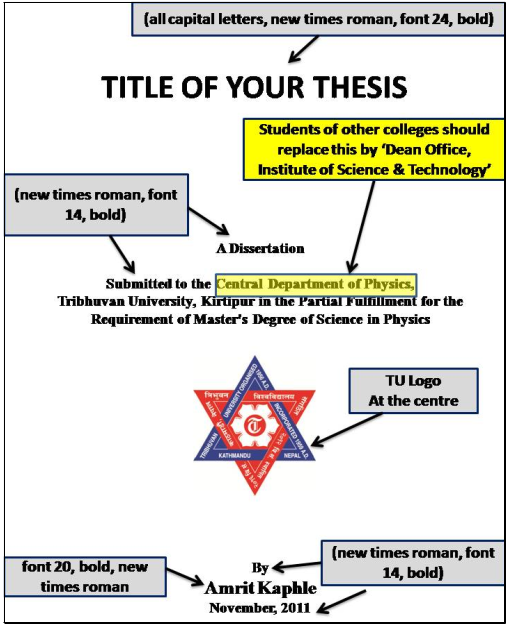
\includegraphics[height=7 cm]{MT}
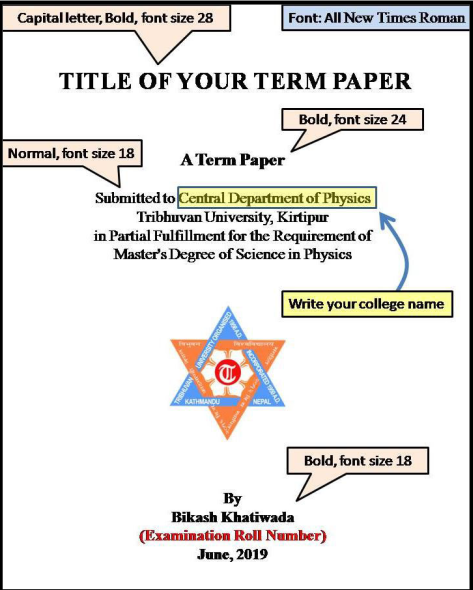
\includegraphics[height=7 cm]{TP}
\end{frame}

	\begin{frame}		
\frametitle{\bf Thesis(Cont..)}
\centering
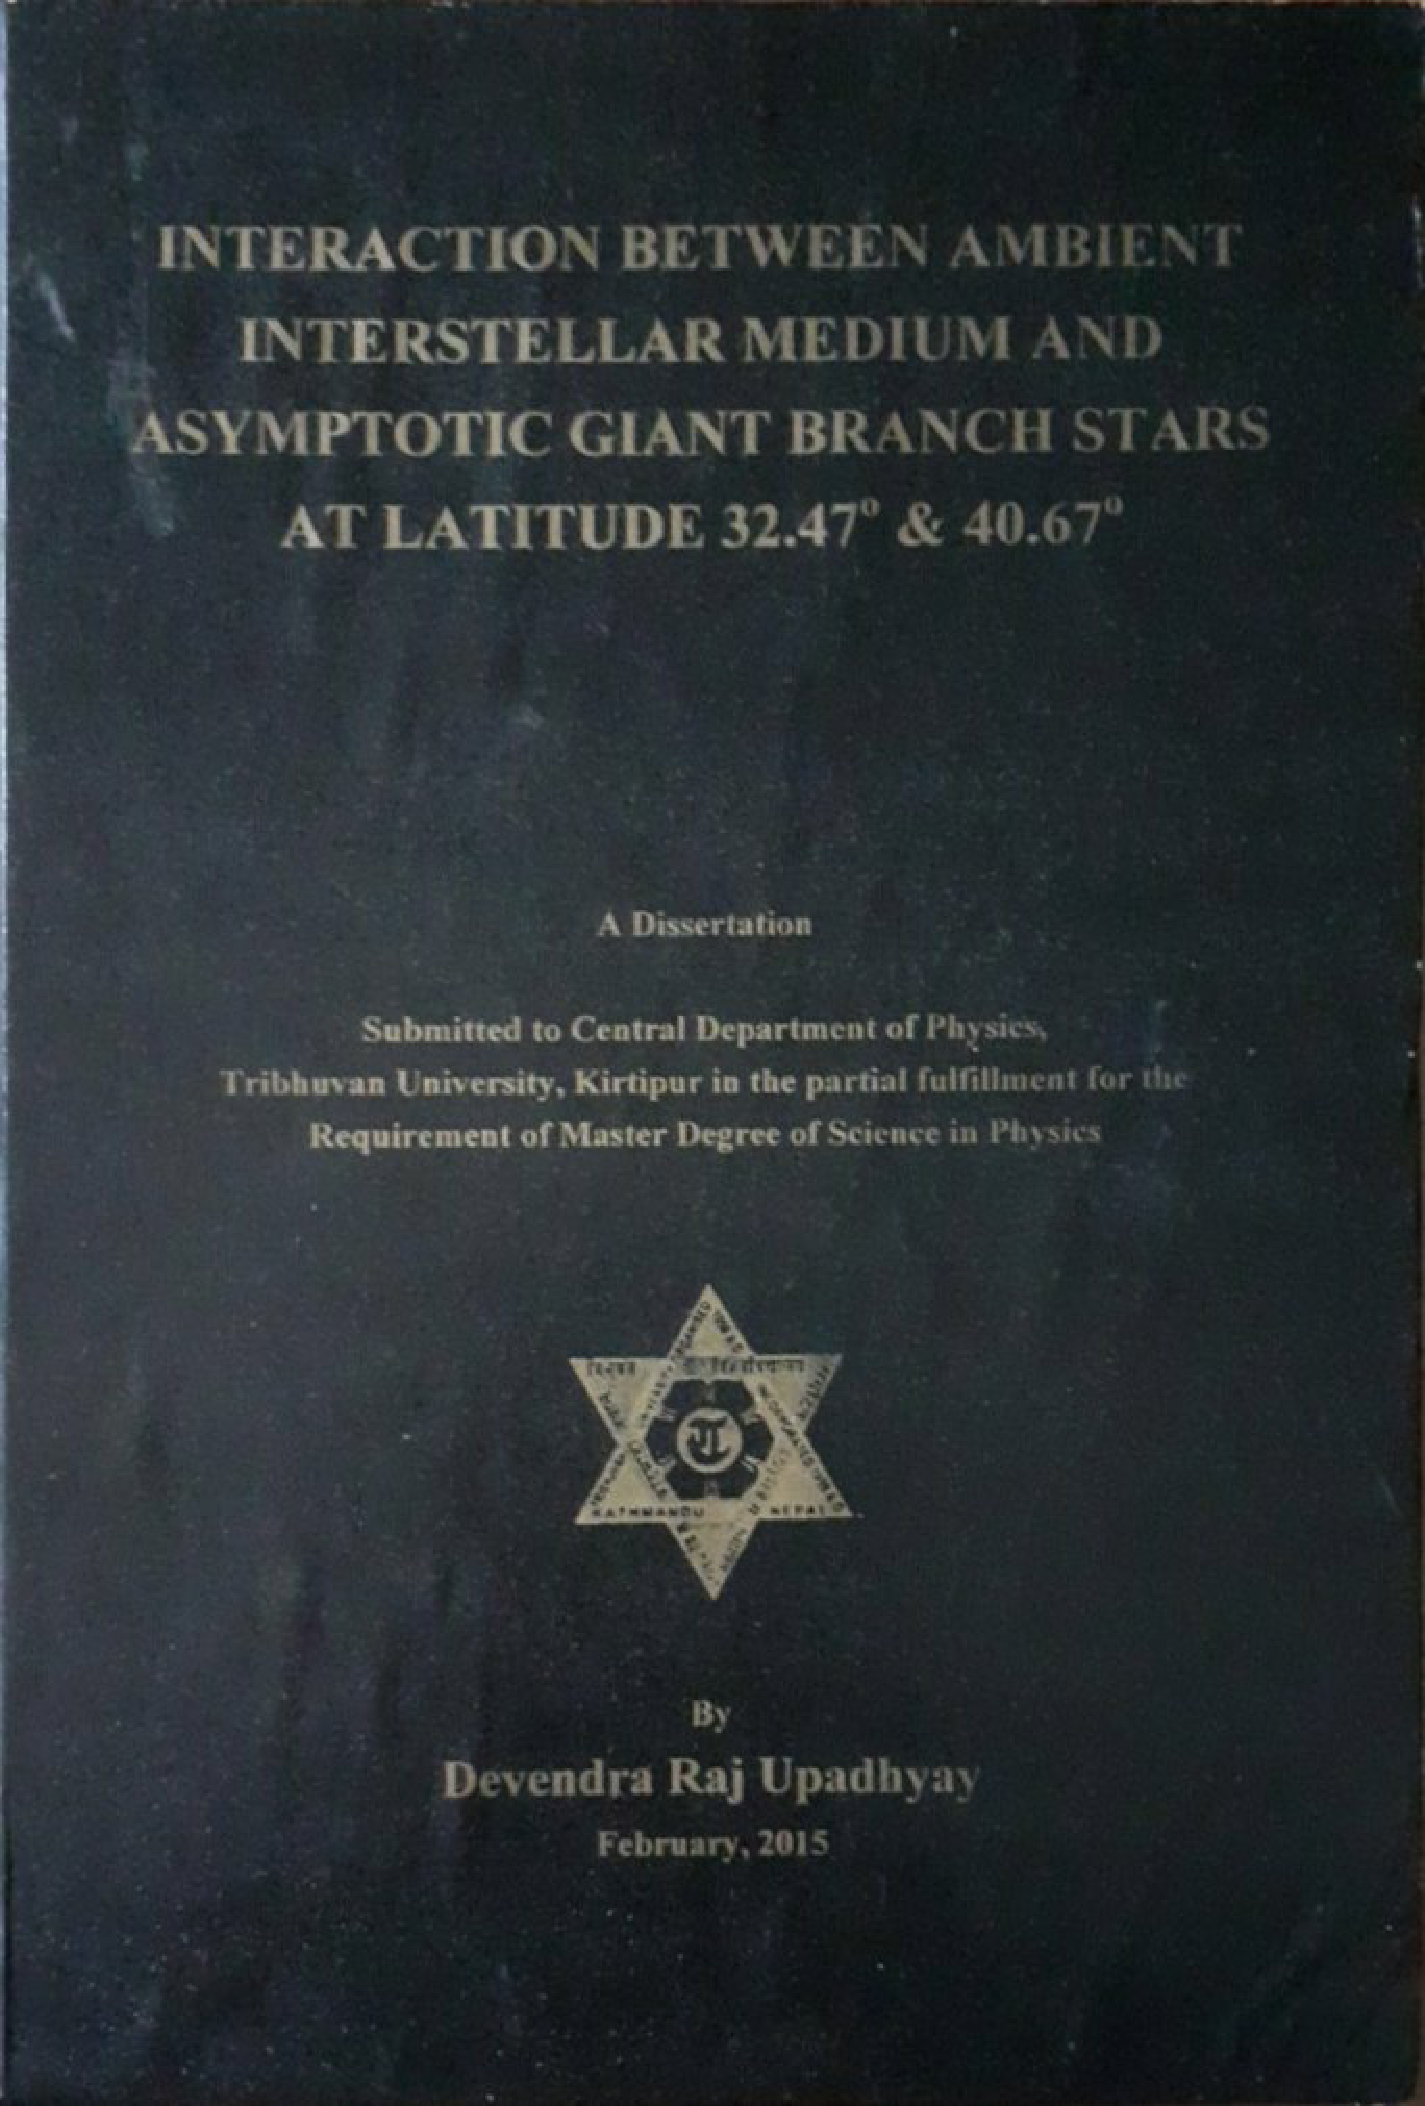
\includegraphics[height=7.5 cm]{T2}
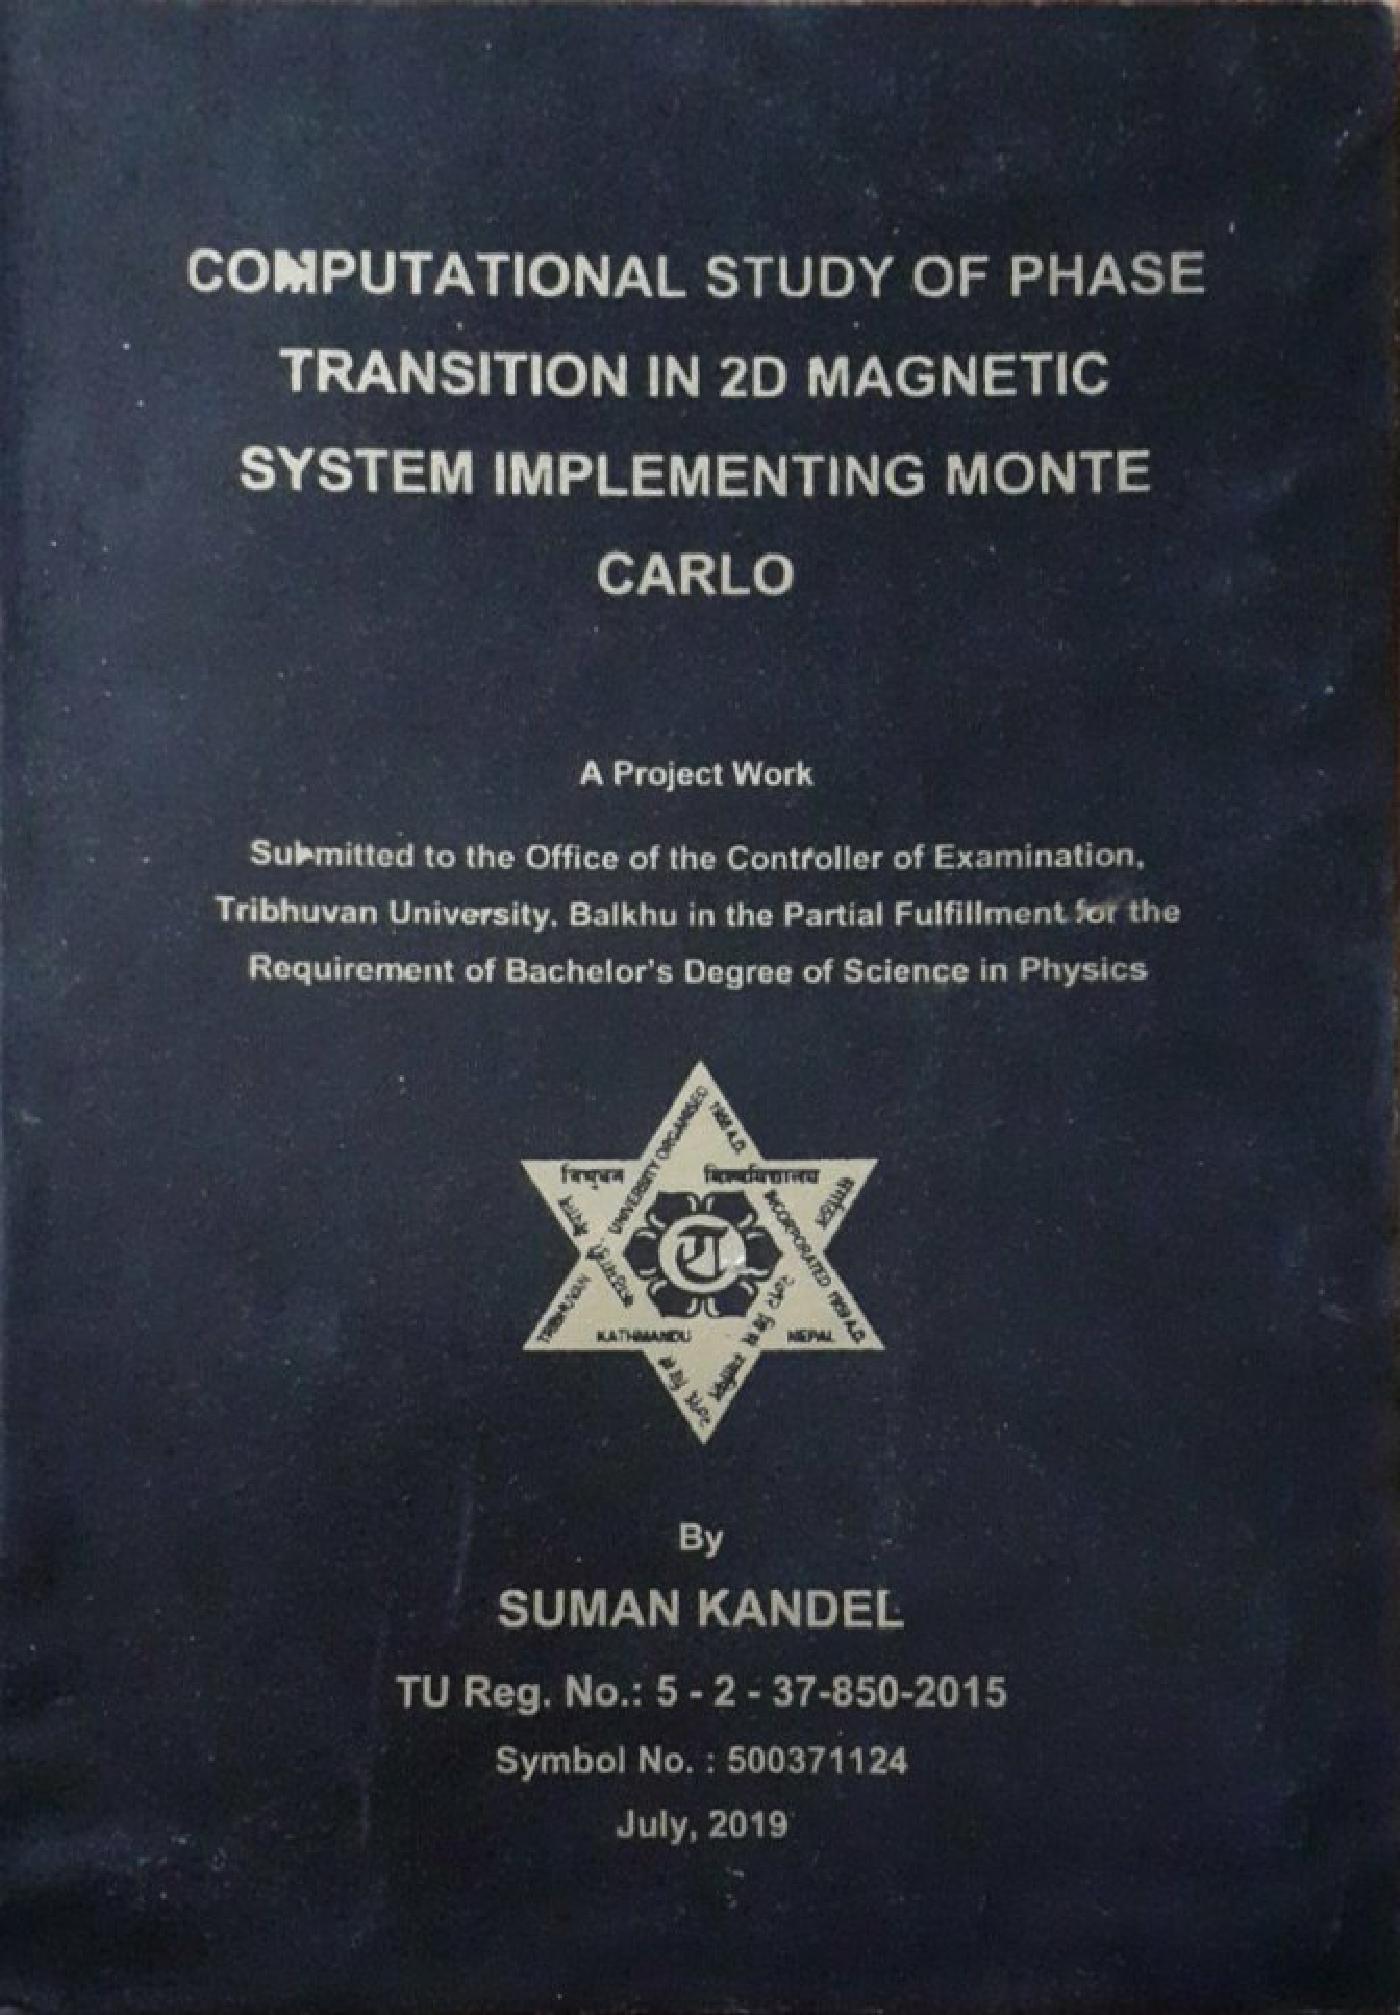
\includegraphics[height=7.5 cm]{T1}
\end{frame}

	\begin{frame}		
\frametitle{\bf WinEdt(Cont..)}
\bf \color{red}WinEdt \bf \color{blue}is a powerful and versatile all-purpose text
editor for Windows with a strong predisposition
towards the creation and compilation of LaTeX
documents...\\
\centering
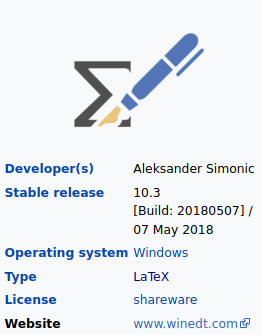
\includegraphics[width=4cm]{WE1}
\footnote{https://www.winedt.com/(April, 2020).}
\footnote{https://en.wikipedia.org/wiki/WinEdt(April, 2020).}
\end{frame}

	\begin{frame}		
\frametitle{\bf WinEdit(Cont..)}
\centering
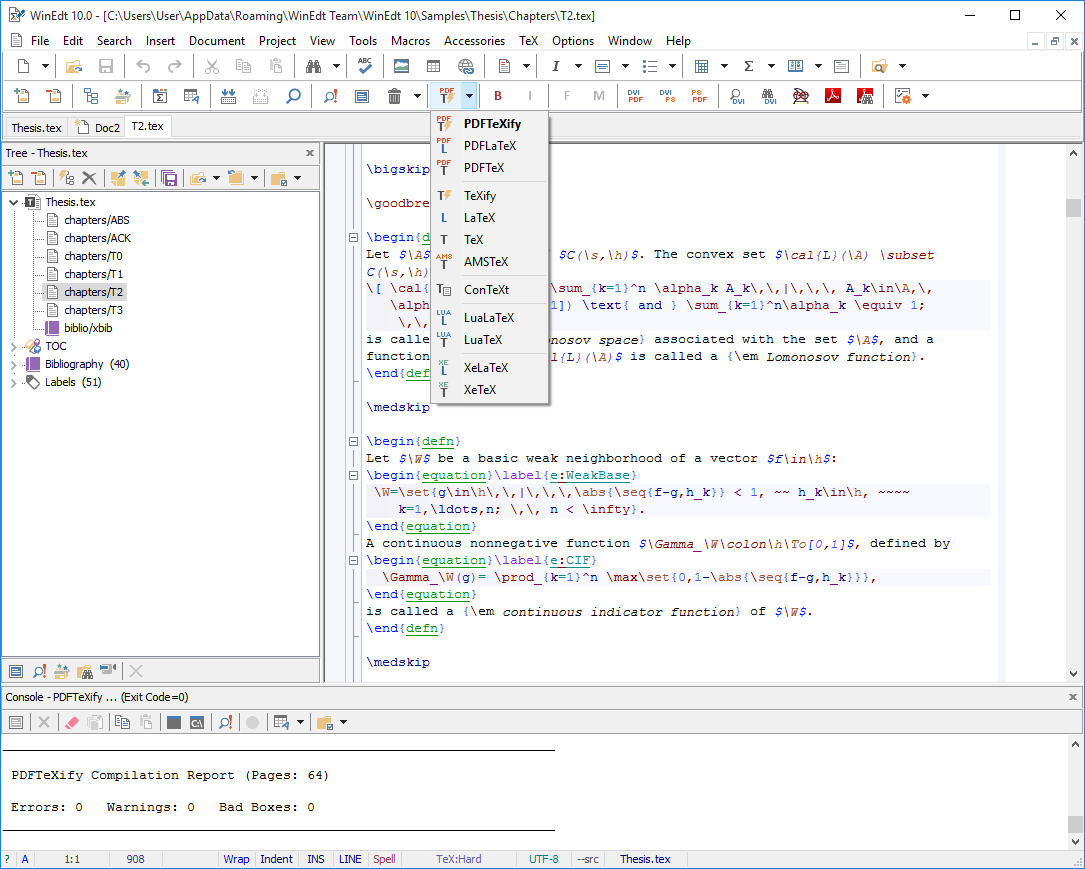
\includegraphics[width=9cm]{WE}
\footnote{https://www.winedt.com/(April, 2020).}	
\end{frame}



\begin{frame}		
\frametitle{\bf Texmaker}
\bf 	\color{red} Texmaker 	\color{blue}is a free, modern and cross-platform LaTeX editor
for linux, macosx and windows systems that integrates many
tools needed to develop documents with LaTeX, in just one
application.
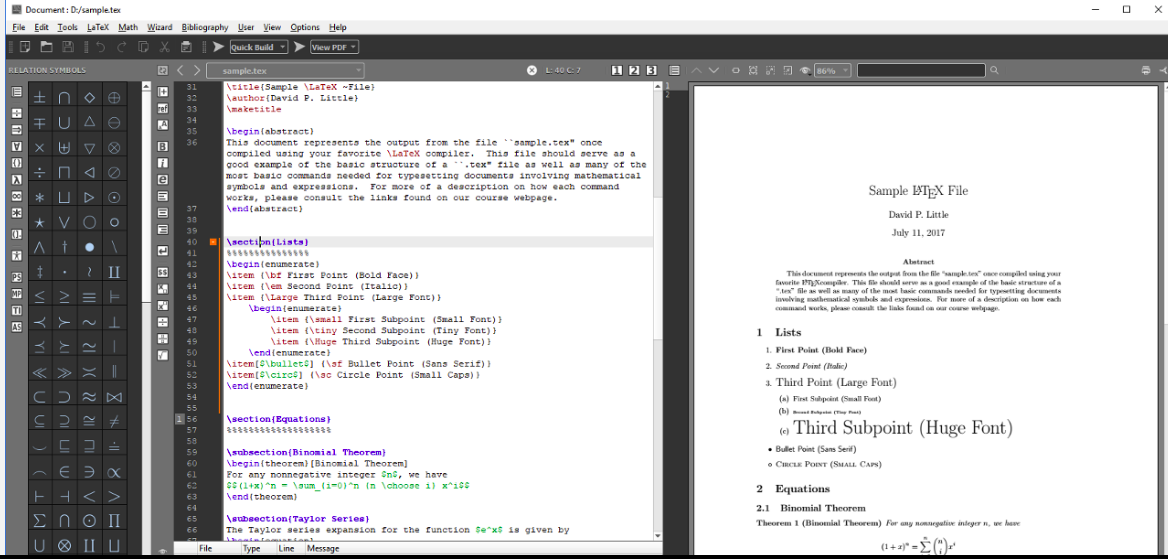
\includegraphics[width=12cm]{Te}
\footnote{https://www.xm1math.net/texmaker/shots.html(April, 2020).}	
\end{frame}





\begin{frame}		
\frametitle{\bf TeXstudio}
\bf 	\color{red} TeXstudio 	\color{blue} is an integrated writing environment for creating LaTeX documents. Our goal is to make writing LaTeX as easy and comfortable as possible. Therefore TeXstudio has numerous features like syntax-highlighting, integrated viewer, reference checking and various assistants. \\
\color{red}
For Ubuntu Linux: \color{blue} Use command\\
sudo apt-get update\\
\color{red}TeXstudio:\color{blue} sudo apt-get install texstudio\\

\color{red}For windows users: \color{blue} download and install\\
\color{red}texstudio: \color{blue} https://texstudio.org/\\
\color{red}miktex:  \color{blue} https://miktex.org/download\\
\footnote{https://www.texstudio.org/(April, 2020).}	
\end{frame}

\begin{frame}
\frametitle{\bf TeXstudio(Thesis/Report)}
\centering
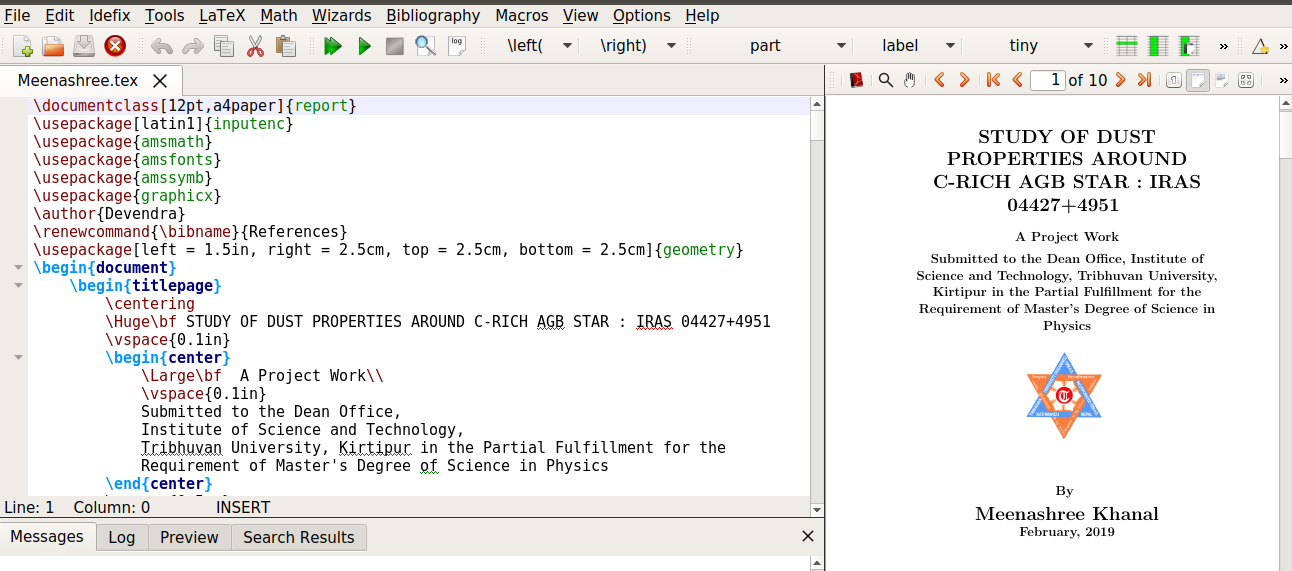
\includegraphics[width=13cm]{Th}
\end{frame}

\begin{frame}
\frametitle{\bf TeXstudio(Thesis/Report)}
\centering
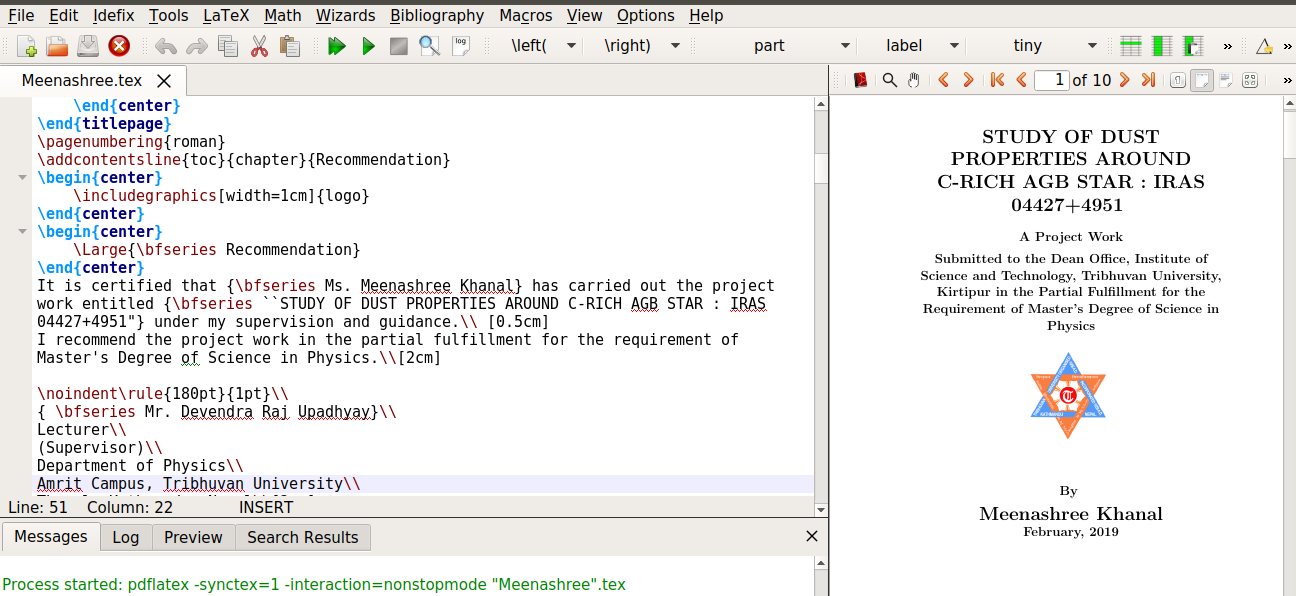
\includegraphics[width=13cm]{Th1}
\end{frame}

\begin{frame}
\frametitle{\bf TeXstudio(Proposal)}
\centering
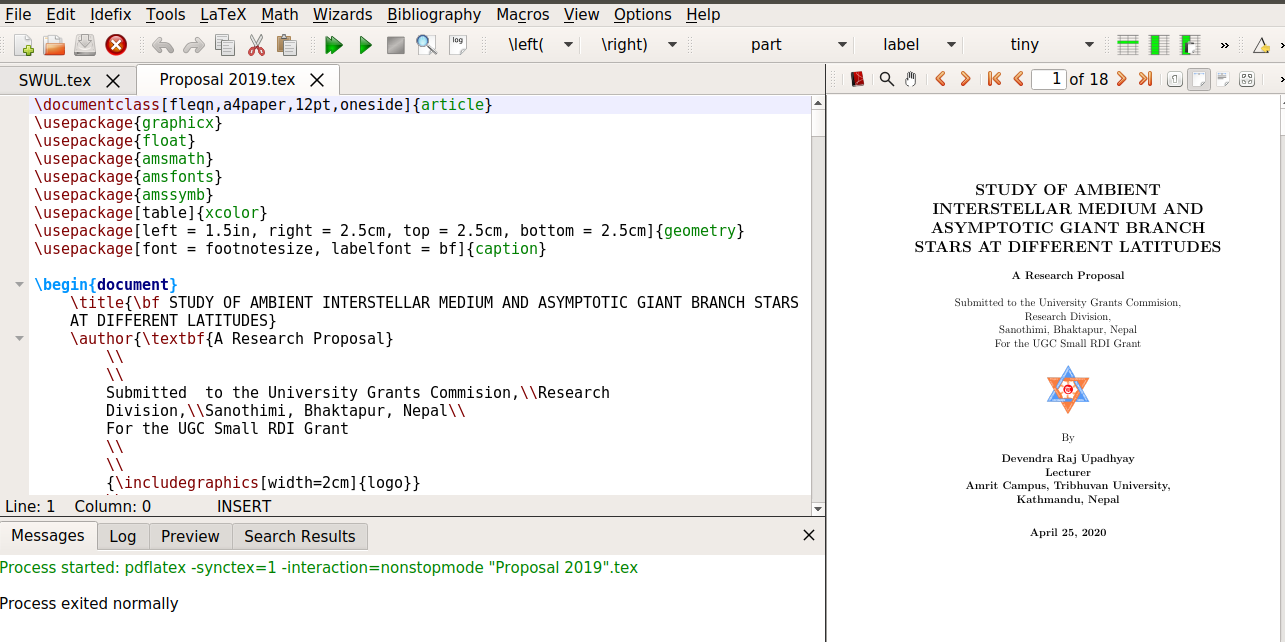
\includegraphics[width=13cm]{Pr}
\end{frame}

\begin{frame}
\frametitle{\bf TeXstudio(Proposal)}
\centering
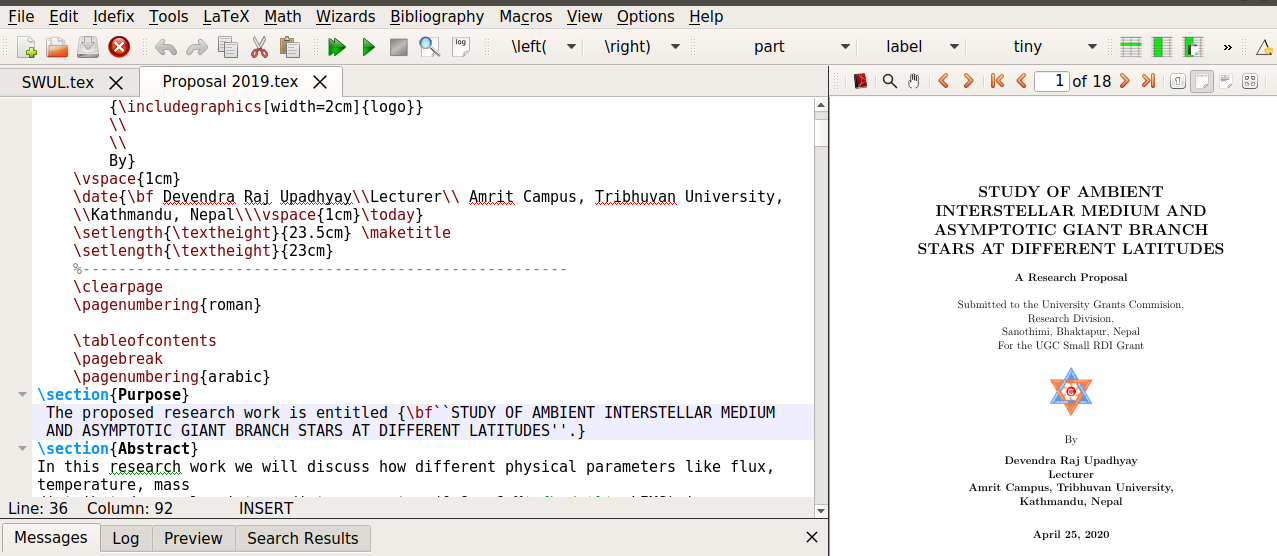
\includegraphics[width=13cm]{Pr1}
\end{frame}


\begin{frame}		
\frametitle{\bf TeXstudio(Beamer Presentation)}
\centering
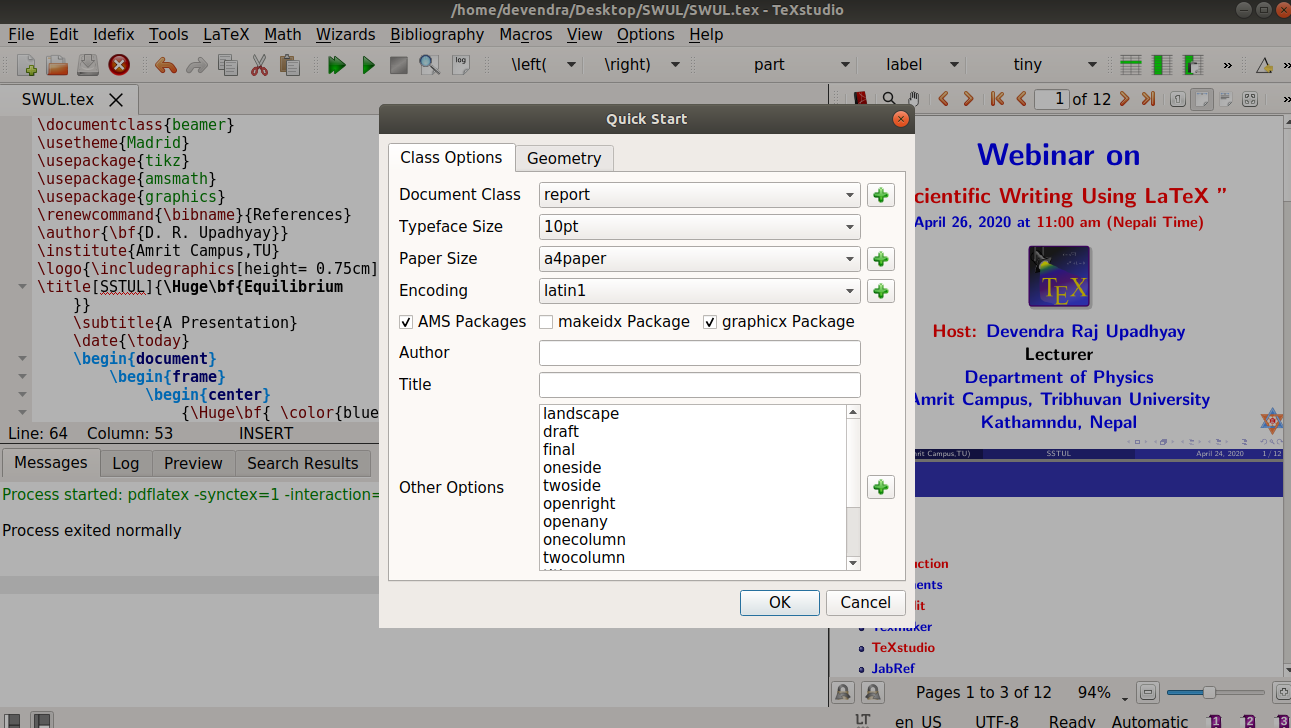
\includegraphics[width=13cm]{TS}
\end{frame}


\begin{frame}		
\frametitle{\bf TeXstudio(Beamer Presentation)}
\centering
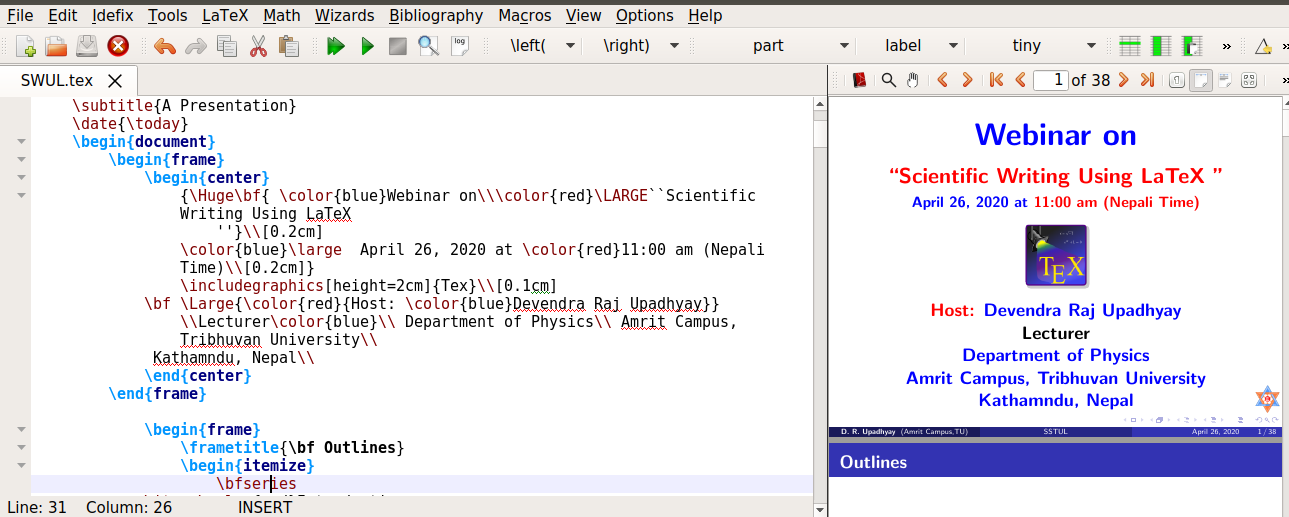
\includegraphics[width=13cm]{Be}
\end{frame}


			\begin{frame}		
		\frametitle{\bf Jabref}
		\bf \color{blue}JabRef is an open source bibliography reference manager. The native
		file format used by JabRef is BibTeX, the standard LaTeX bibliography
		format. JabRef is a desktop application and runs on the Java VM
		(version 8), and works equally well on Windows, Linux, and Mac OS X.\\\vspace{1cm}
		\bf
		 \color{red}For Windows \& Mac OS: \color{blue} download and install them\\
		 	\begin{itemize}
		 	
		 	\bfseries
		 	\item \color{red}Jabref: \color{blue} http://www.jabref.org/
		 		 
		 	
		 \end{itemize}
	 	\color{red} For Ubuntu Linux:
		\begin{itemize}
			
		
			\item \color{blue} Step 1: sudo apt-get update -y
			\item \color{blue} Step 2: sudo apt-get install -y jabref
			
		\end{itemize}
		
	\end{frame}

	\begin{frame}		
\frametitle{\bf Jabref}
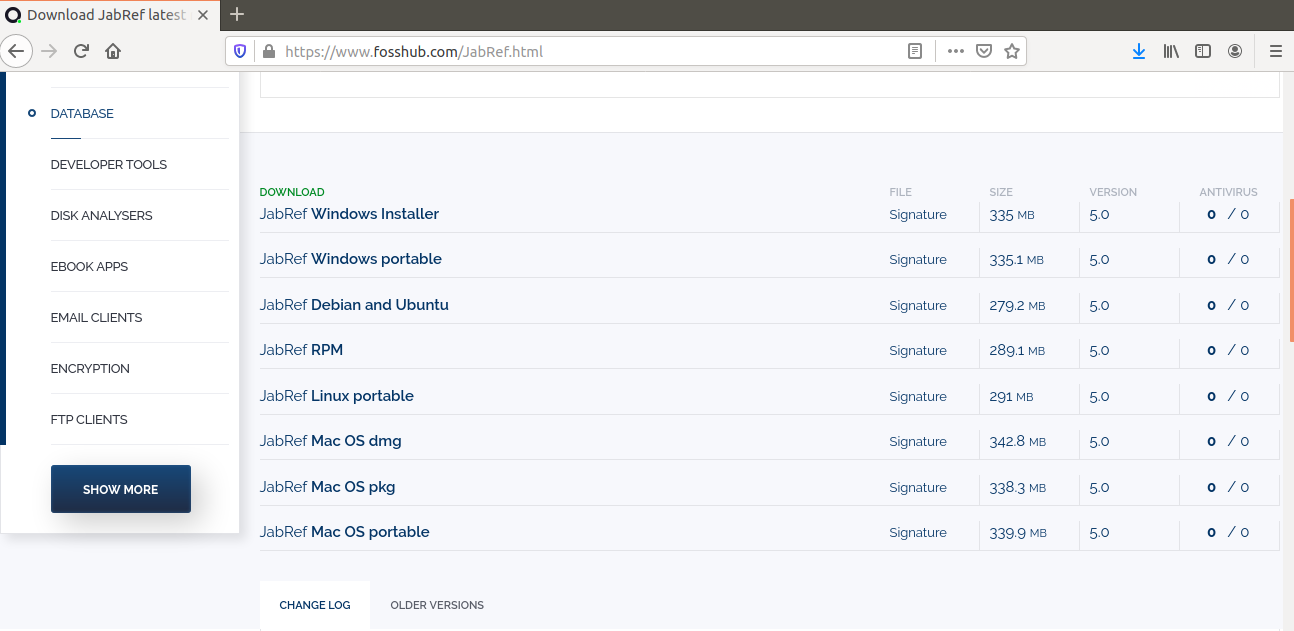
\includegraphics[width=12cm]{JR1}
\footnotetext{text}	
\end{frame}
			
				\begin{frame}		
			\frametitle{\bf Jabref}
		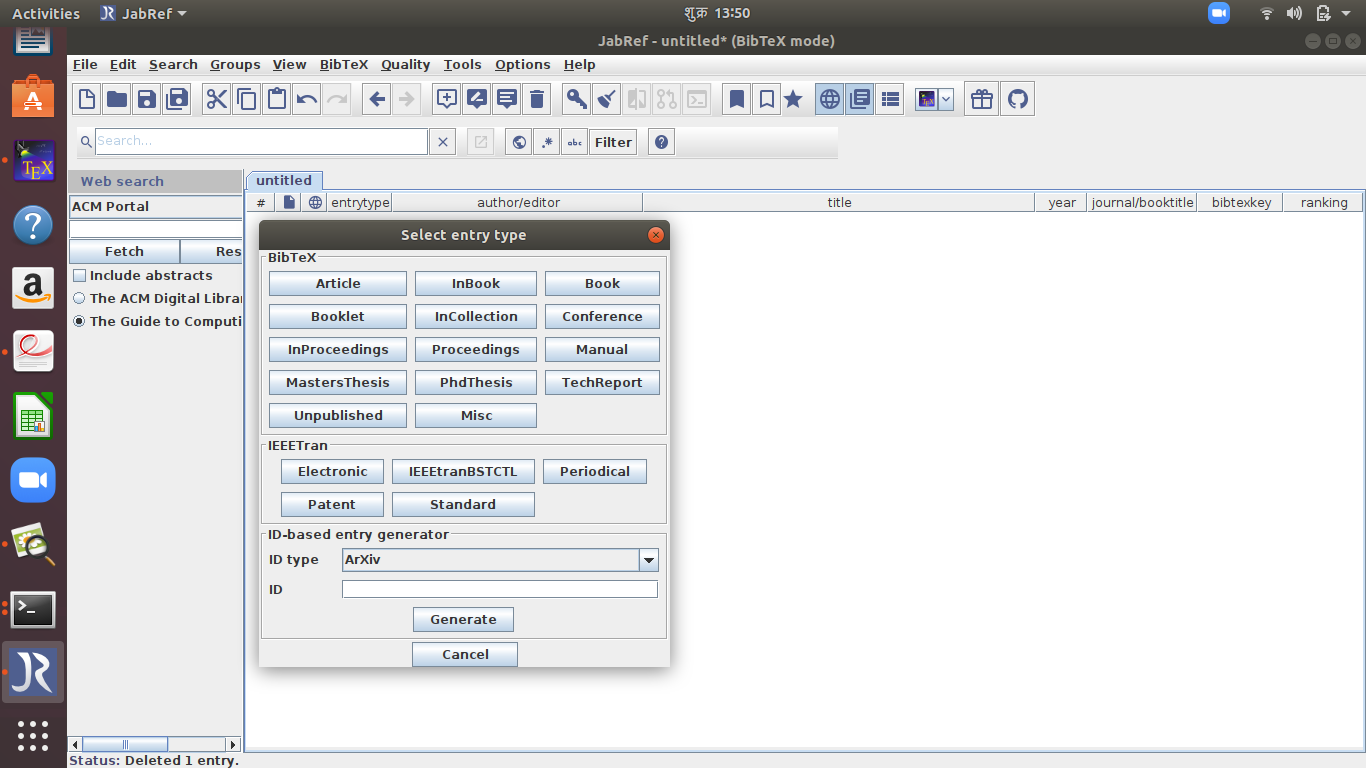
\includegraphics[width=12cm]{JR}	
		\end{frame}
	\begin{frame}
	\frametitle{\bf Special Characters}
		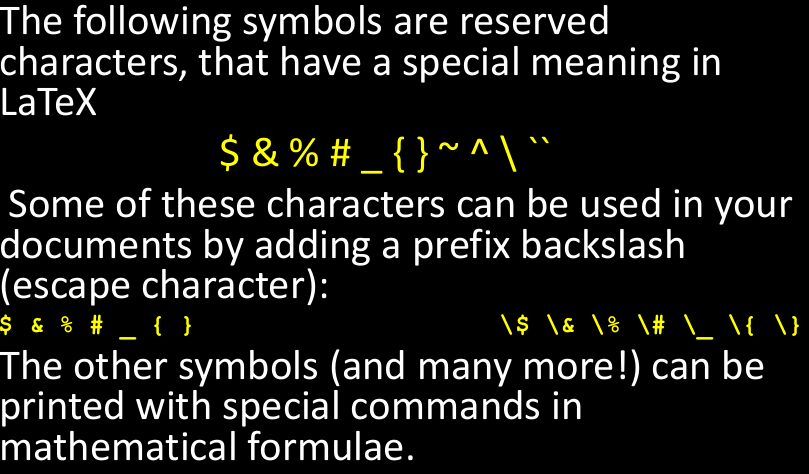
\includegraphics[width=12cm]{SY}
	\end{frame}

	\begin{frame}
\frametitle{\bf How to type Mathematics}
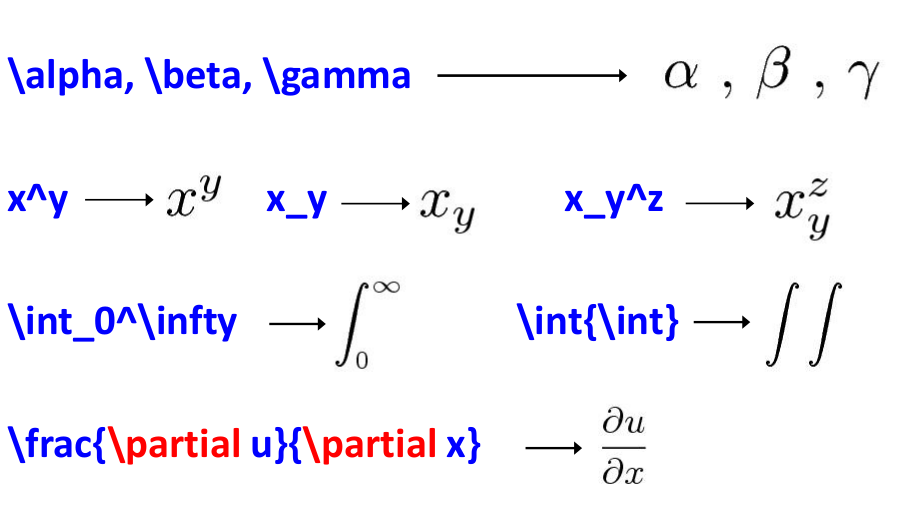
\includegraphics[width=12cm]{HM}
\end{frame}
		\begin{frame}		
	\frametitle{\bf Typesetting Equations}
		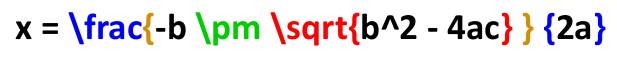
\includegraphics[width=12cm]{EQ1}

		This is my solution

	$\large	\bf \color{red} x = \frac{-b \pm \sqrt{b^2 - 4ac} } {2a}$
	
		\begin{equation}
		\frac{d^2\psi}{dx^2} + \frac{2m}{\hbar^2}(E - V)\psi = 0
		\end{equation}
		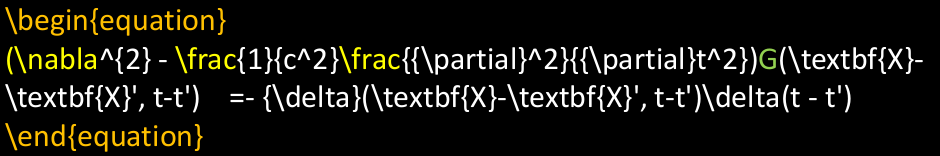
\includegraphics[width=12cm]{EQ}
		\begin{equation}
		\large	\bf \color{red} (\nabla^{2} - \frac{1}{c^2}\frac{{\partial}^2}{{\partial}t^2})G(\textbf{X}-
			\textbf{X}', t-t') =- {\delta}(\textbf{X}-\textbf{X}', t-t')\delta(t - t')
		\end{equation}
		
	\end{frame}	
			\begin{frame}		
		\frametitle{\bf Matrix}	
		\bf \color{red}The \emph{characteristic polynomial} $\chi(\lambda)$ of the
		$3 \times 3$~matrix
		\color{blue}
		\[ \left( \begin{array}{ccc}
		a & b & c \\
		d & e & f \\
		g & h & i \end{array} \right)\]
	\bf \color{red}	is given by the formula
		\[ \chi(\lambda) = \left| \begin{array}{ccc}
		\lambda - a & -b & -c \\
		-d & \lambda - e & -f \\
		-g & -h & \lambda - i \end{array} \right|.\]
			\end{frame}	
			\begin{frame}
		\frametitle{\bf Chemical Reaction}
		\centering 
		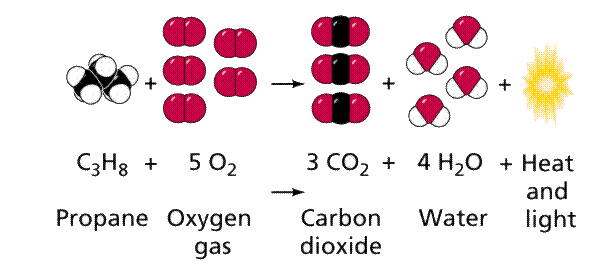
\includegraphics[width=10cm]{CR}
		\bf \large  \color{blue} $C_{3}H_{8} + 5 O_{2} \xrightarrow{\hspace*{1cm}} 3 CO_{2} + 4 H_{2}O +$ Heat and light
		\begin{equation}
		\bf \large  \color{red} C_{3}H_{8} + 5 O_{2} \xrightarrow{\hspace*{1cm}} 3 CO_{2} + 4 H_{2}O + Heat\hspace{0.1cm} and \hspace{0.1cm} light
		\end{equation}
	
	\end{frame}	
			\begin{frame}
			\frametitle{\bf Figure/Image}
	\color{red}	First load the package graphics: 	\color{blue}	usepackage ${graphicx}$
		\color{red}	Then include the figure like this:
		\begin{figure}
			\centering
			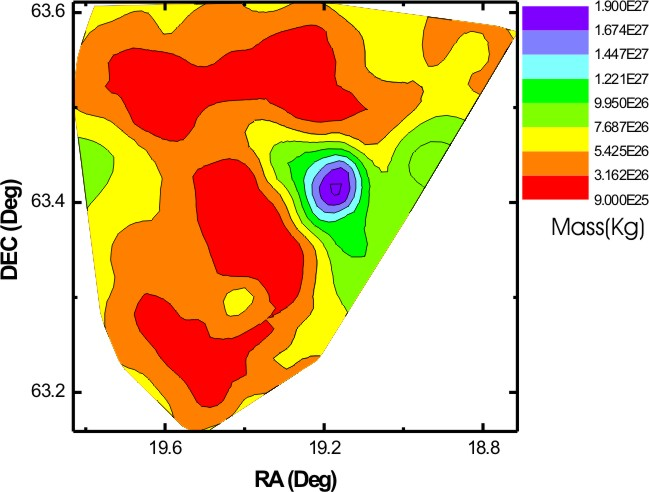
\includegraphics[width = 6cm]{Cm}
			\caption{Dust mass contour map.}
		\end{figure}
		\end{frame}	
	
		\begin{frame}
	\frametitle{\bf Drawing}
	\centering
	
	\begin{tikzpicture}
	\draw (0,0) -- (4,0) -- (4,4) -- (0,4) -- (0,0);
	\end{tikzpicture}
	
	
	\begin{tikzpicture}
	\draw (2,2) circle (2cm);
	\end{tikzpicture}
	
\end{frame}


\begin{frame}
\frametitle{\bf Graph ???}

\begin{tikzpicture}
\draw[thick,->] (0,0) -- (4.5,0) node[anchor=north west] {x axis};
\draw[thick,->] (0,0) -- (0,4.5) node[anchor=south east] {y axis};
<code goes here>\foreach \x in {0,1,2,3,4}
\draw (\x cm,1pt) -- (\x cm,-1pt) node[anchor=north] {$\x$};
\foreach \y in {0,1,2,3,4}
\draw (1pt,\y cm) -- (-1pt,\y cm) node[anchor=east] {$\y$};
\end{tikzpicture}

\footnote{https://www.overleaf.com/learn(April, 2020).}
\end{frame}

	\begin{frame}
	\frametitle{\bf Circuit Diagrams}
	\centering
\begin{circuitikz}
	\draw
	%(0,0) to[R, o-o] (2,0)
%	(4,0) to[vR, o-o] (6,0)
	%(0,2) to[transmission line, o-o] (2,2)
	(4,2) to[closing switch, o-o] (6,2)
	(0,4) to[european current source, o-o] (2,4)
	(4,4) to[european voltage source, o-o] (6,4)
	(0,6) to[empty diode, o-o] (2,6)
	(4,6) to[full led, o-o] (6,6)
	(0,8) to[generic, o-o] (2,8)
	(4,8) to[sinusoidal voltage source, o-o] (6,8);
\end{circuitikz}
\end{frame}

\begin{frame}
\frametitle{\bf Circuit}
\centering 
\begin{circuitikz} \draw
(0,0) to[battery] (0,4)
to[ammeter] (4,4) -- (4,0)
to[lamp] (0,0)
(0.5,0) -- (0.5,-2)
to[voltmeter] (3.5,-2) -- (3.5,0)
;
\end{circuitikz}
\end{frame}


	\begin{frame}
	\frametitle{\bf Grant Chart and Detailed Budget}
	\begin{table}[h]
		\centering
		\caption{The expected budget for the proposed research program has been estimated as
			follows:}
		\vspace{1 pt}
		\begin{tabular}{||c|c|c||}
			\hline
			\hline
			\textbf{S.N.} & \textbf{Particulars} & \textbf{Estimated Budget}\\
			& & \textbf{(Rs.)}\\
			\hline
			\hline
			1.	& Reference Books & 45,000\\
			    &/Journals/Documents and Stationary & \\
			\hline
			2. &  Library fee & 50000 \\
			\hline
			3. &  Scientific tools, genuine software & 100,000 \\
			\hline
			\hline
		\end{tabular}
		\label{Engpb} \end{table}
	\end{frame}	

\begin{frame}
\frametitle{\bf Font Size}
\vspace*{0cm}
\centering
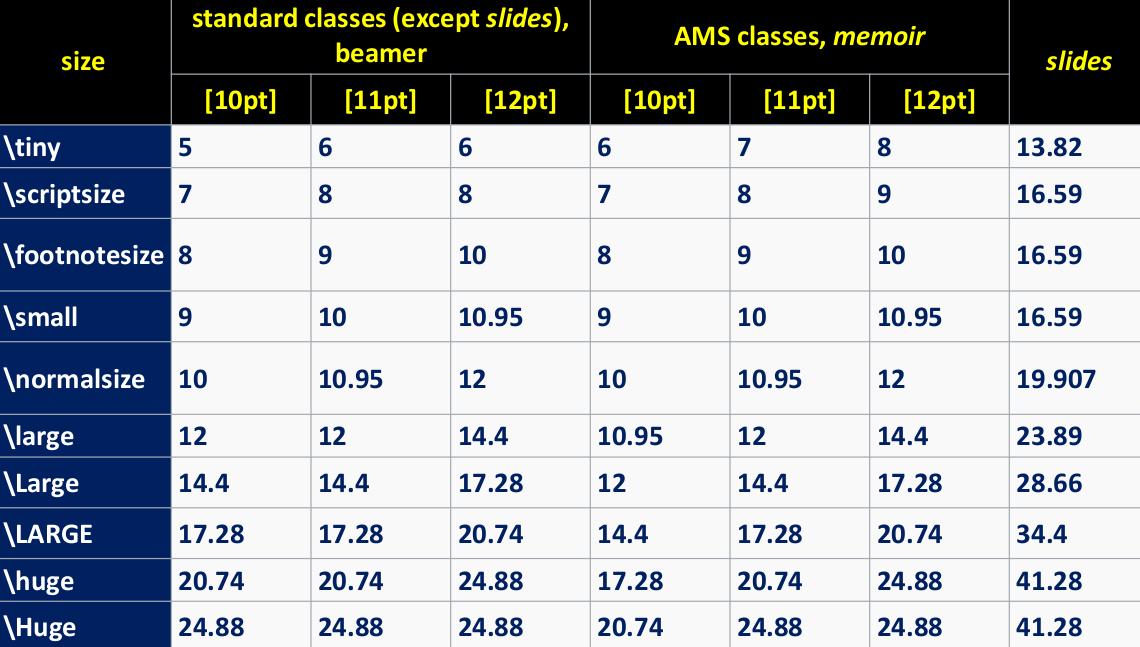
\includegraphics[width=12cm]{FS}
\end{frame}


\begin{frame}
\frametitle{\bf Research Missconduct}
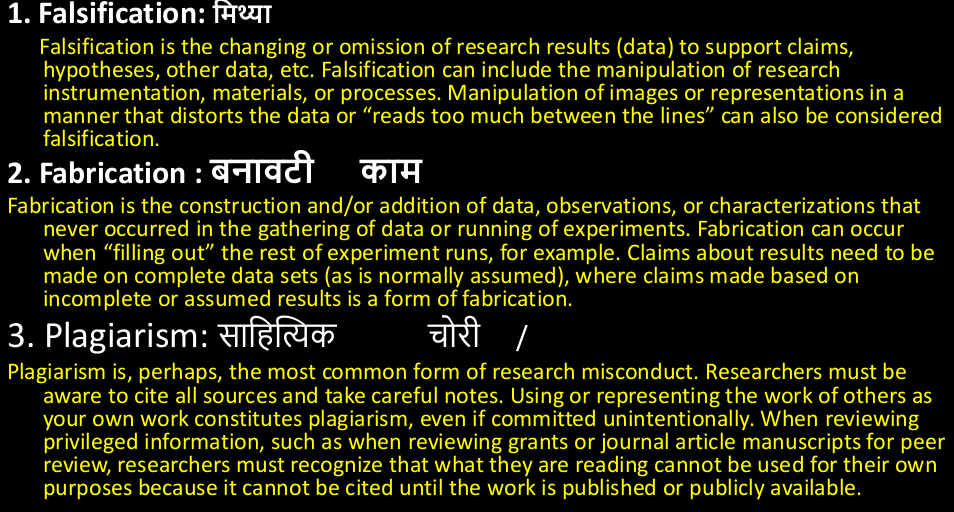
\includegraphics[width=12cm]{MC}\footnote{Gilbert, F. J., \& Denison, A. R. (2003). Research Misconduct. Clinical Radiology, 58(7), 499–504. doi:10.1016/s0009-9260(03)00176-4 }
\end{frame}

\begin{frame}
\frametitle{\bf References \& Citation}
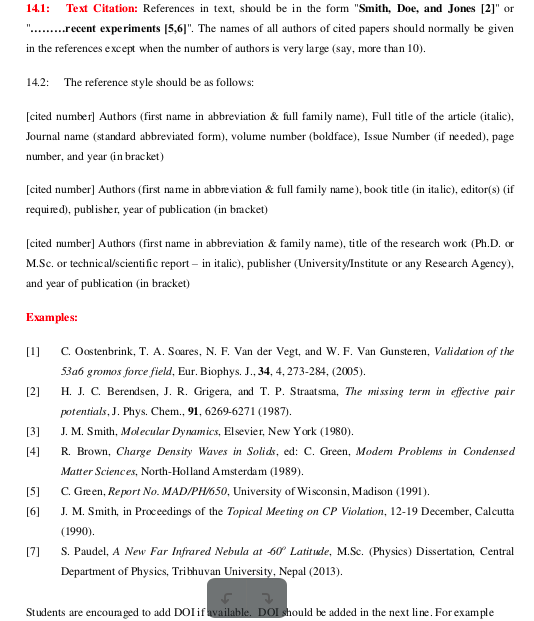
\includegraphics[width=6cm]{RS1}

\includegraphics[width=5cm]{RS}
\end{frame}
\begin{frame}
\frametitle{\bf References \& Citation}
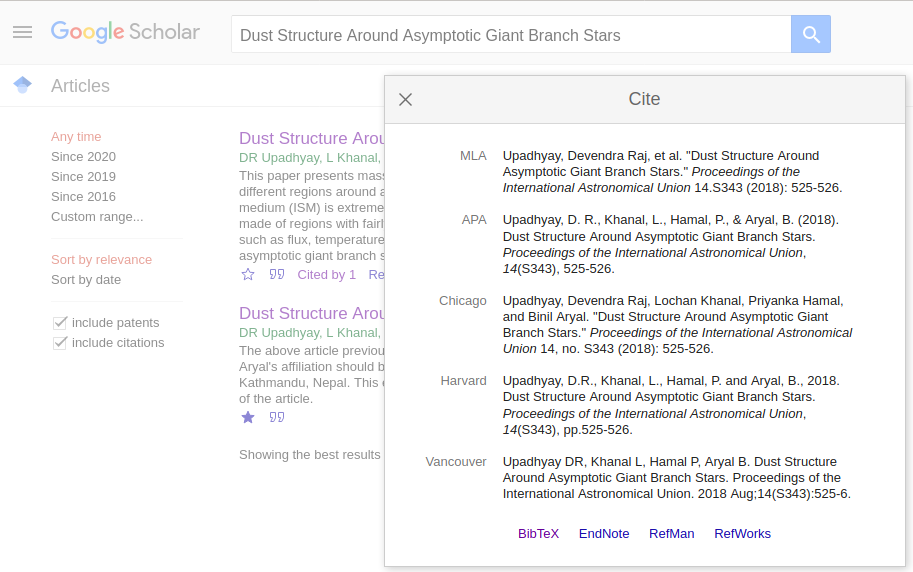
\includegraphics[width=5.5cm]{GS}
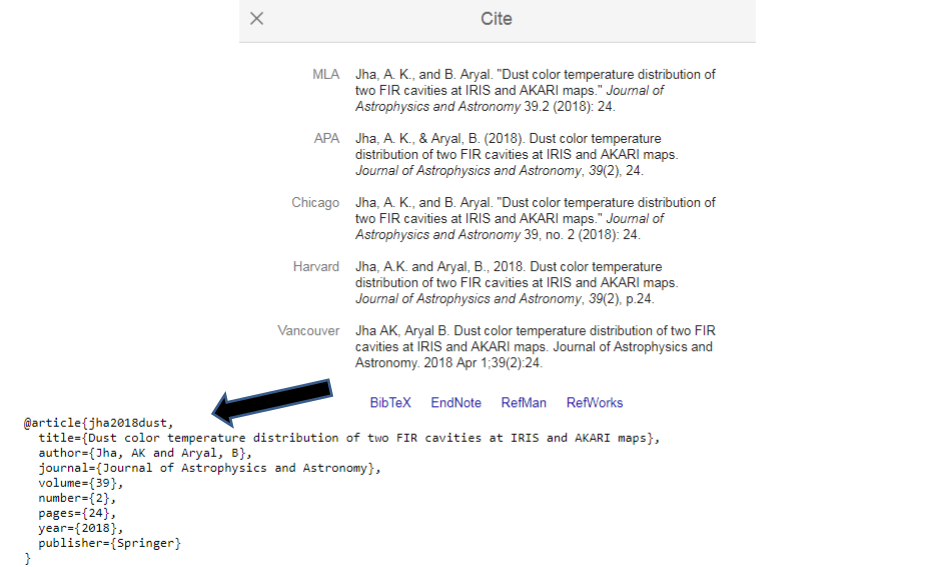
\includegraphics[width=5.5cm]{GS1}
\end{frame}

\begin{frame}
\frametitle{\bf References \& Citation}
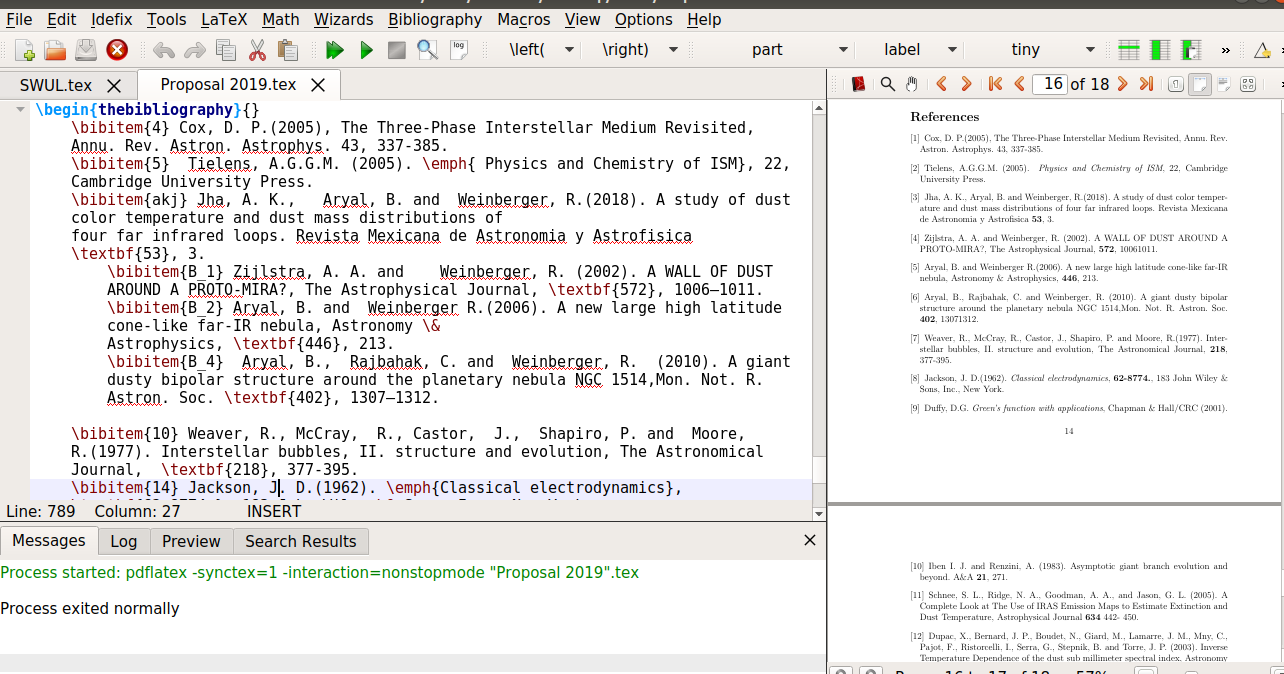
\includegraphics[width=12cm]{RE}
\end{frame}
\begin{frame}
\frametitle{\bf References \& Citation}
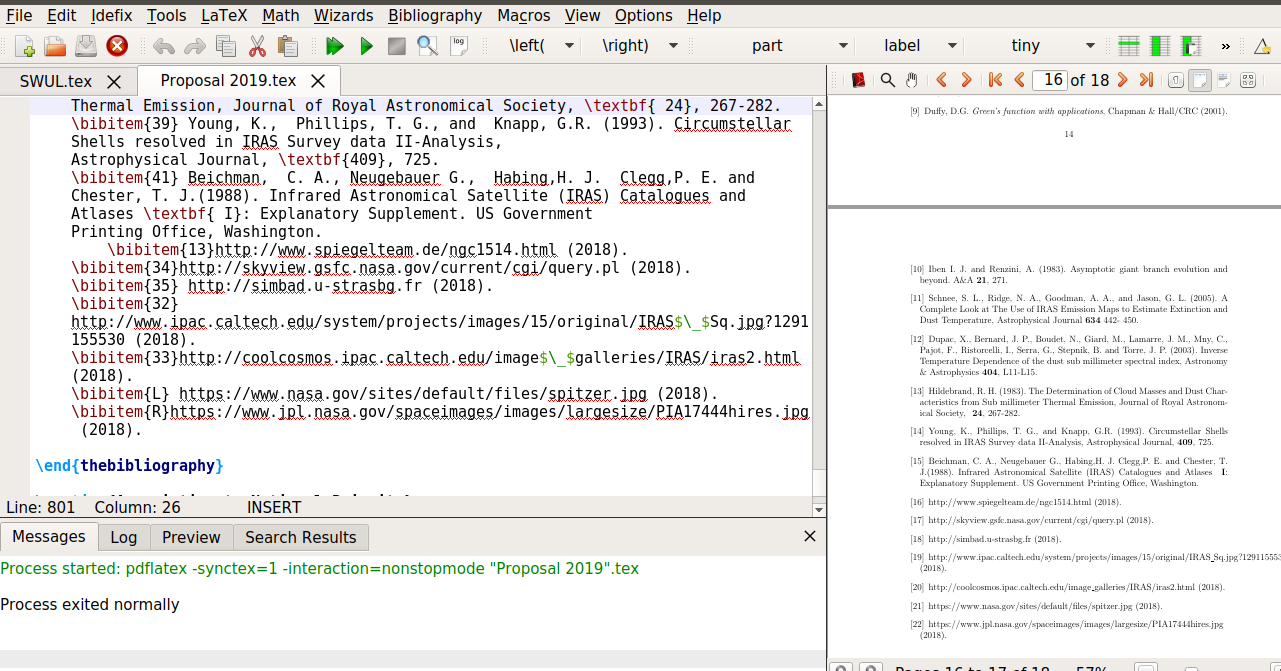
\includegraphics[width=12cm]{RE1}
\end{frame}

\begin{frame}
\frametitle{\bf Home Work (Proposal Writing)}
\begin{itemize}
	\bf
	\item \color{red}Everybody talking about economy crisis these days in
	Nepal. Develop a research proposal requesting for research grant
	to the Research Division of Tribhuvan University on one of the
	topics related to the economy growth of country like Nepal.
	\item \color{blue} Modern era is the science and technology era Need of
	supercomputer is essential in your physics department.
	Develop a research proposal requesting for grant to the
	Research Division of University Grant Commission.
	\item  \color{red} Develop a proposal with essential components for M.Sc.
	Thesis on any relevant topic related to Interstellar Medium to B.P.
	Koirala Memorial Planetarium, Science Museum development Board,
\end{itemize}
\end{frame}

\begin{frame}
\frametitle{\bf Home Work (Proposal Writing)}
\begin{itemize}
\bf
\item \color{blue} Develop a proposal with essential components for M.Sc.
Thesis on any relevant topic related to Galaxy Evolution to
Nepal Academy of Science \& Technology Khumaltar,
Lalitpur, Nepal.\\
\item \color{red}Develop a proposal with essential components any
relevant topic related to Need of Entrepreneurship for
Physicists to Research Division of Institute of Science and
Technology, Tribhuvan University, Nepal.
\end{itemize}
\end{frame}

%\begin{frame}
%\vspace{6cm}
%\centering
%\bf\Large\color{red}{Questions ???}\color{black}
%
%\end{frame}

\begin{frame}
\centering
\Huge\bf\color{red}{Thank You Very Much!!!}\\
\vspace{4cm}
\bf\large\color{blue}{[Take Care, Stay Safe \& Stay busy in Research]}
\end{frame}

\end{document}

